\section{Manual de usuario}

\subsection{Introducción} 
Se ha integrado en la aplicación JMR una nueva funcionalidad que permite a los usuarios generar imágenes a partir de descripciones textuales de forma sencilla y eficiente. Este módulo utiliza algoritmos avanzados de inteligencia artificial para interpretar el texto y transformarlo en contenido visual.

Con esta funcionalidad, puedes:
\begin{itemize}
    \item Generar imágenes directamente desde descripciones en lenguaje natural.
    \item Consultar imágenes generadas previamente sin mostrarlas directamente en pantalla.
    \item Guardar las imágenes generadas para su uso posterior.
\end{itemize}

Este manual proporciona una guía paso a paso para utilizar esta funcionalidad, e incluye ejemplos prácticos y una descripción detallada de cada acción disponible en la interfaz.

\subsection{Inicio de la aplicación}
\begin{enumerate}
    \item Abre la aplicación JMR haciendo clic en el icono correspondiente en tu escritorio o desde el menú de inicio de tu sistema operativo.
    \item Una vez abierta, observarás la interfaz principal de JMR, donde se encuentran las dos nuevas funcionalidades de generación de imágenes.
\end{enumerate}

\begin{figure}[H]
    \centering
    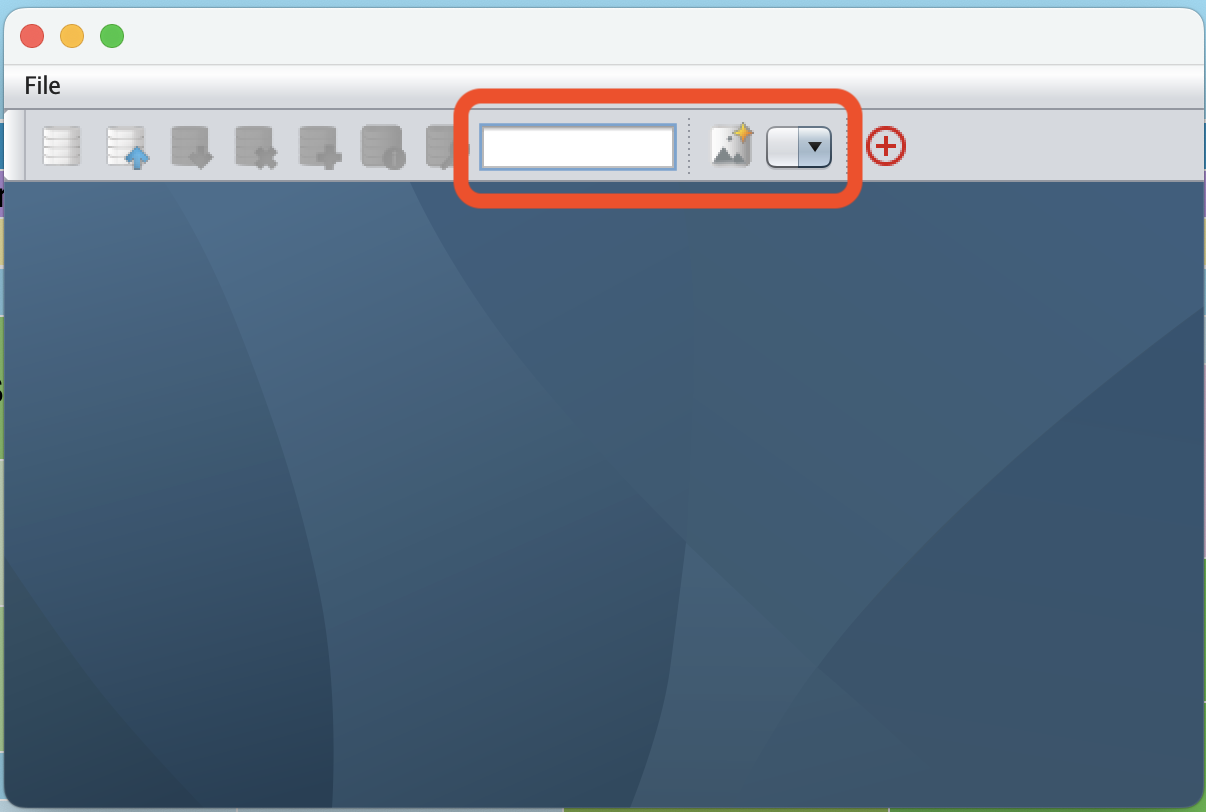
\includegraphics[width=0.5\textwidth]{manual/captura1.png}
    \caption{Inicio de la aplicación con las dos nuevas funcionalidades}
    \label{fig:inicio}
\end{figure}

\subsection{Descripción de la interfaz} 
Las nuevas funcionalidades de generación de imágenes están integradas en la barra superior y presentan los siguientes elementos:
\begin{enumerate}
    \item \textbf{Cuadro de texto}: Espacio donde puedes escribir la descripción textual de la imagen que deseas buscar en la base de datos.
    \item \textbf{Generar imagen}: Abre una ventana con un área de texto en la que puedes describir la imagen a generar. Dentro de esta hay un botón para generar y visualizar la imagen descrita.
    \item \textbf{Lista desplegable}: Lista desplegable que muestra un historial de las imágenes generadas junto a sus descripciones. Permite seleccionar una entrada anterior para visualizarla nuevamente.
\end{enumerate}

A continuación, se detallan las funcionalidades específicas de generación y búsqueda.


\subsection{Cómo generar una imagen}
Para generar una nueva imagen a partir de una descripción textual, sigue los siguientes pasos:

\textbf{Paso 1: Acceder al generador}
\begin{enumerate}
    \item Haz clic en el botón \textit{Generar Imagen}, situado en la barra superior de la aplicación.
    \item Se abrirá una ventana interna que contiene:
    \begin{itemize}
        \item Un cuadro de texto para introducir la descripción.
        \item Una imagen por defecto como marcador de posición.
        \item Un botón con la etiqueta \textit{Visualizar Imagen}.
    \end{itemize}
    
    \begin{figure}[H]
        \centering
        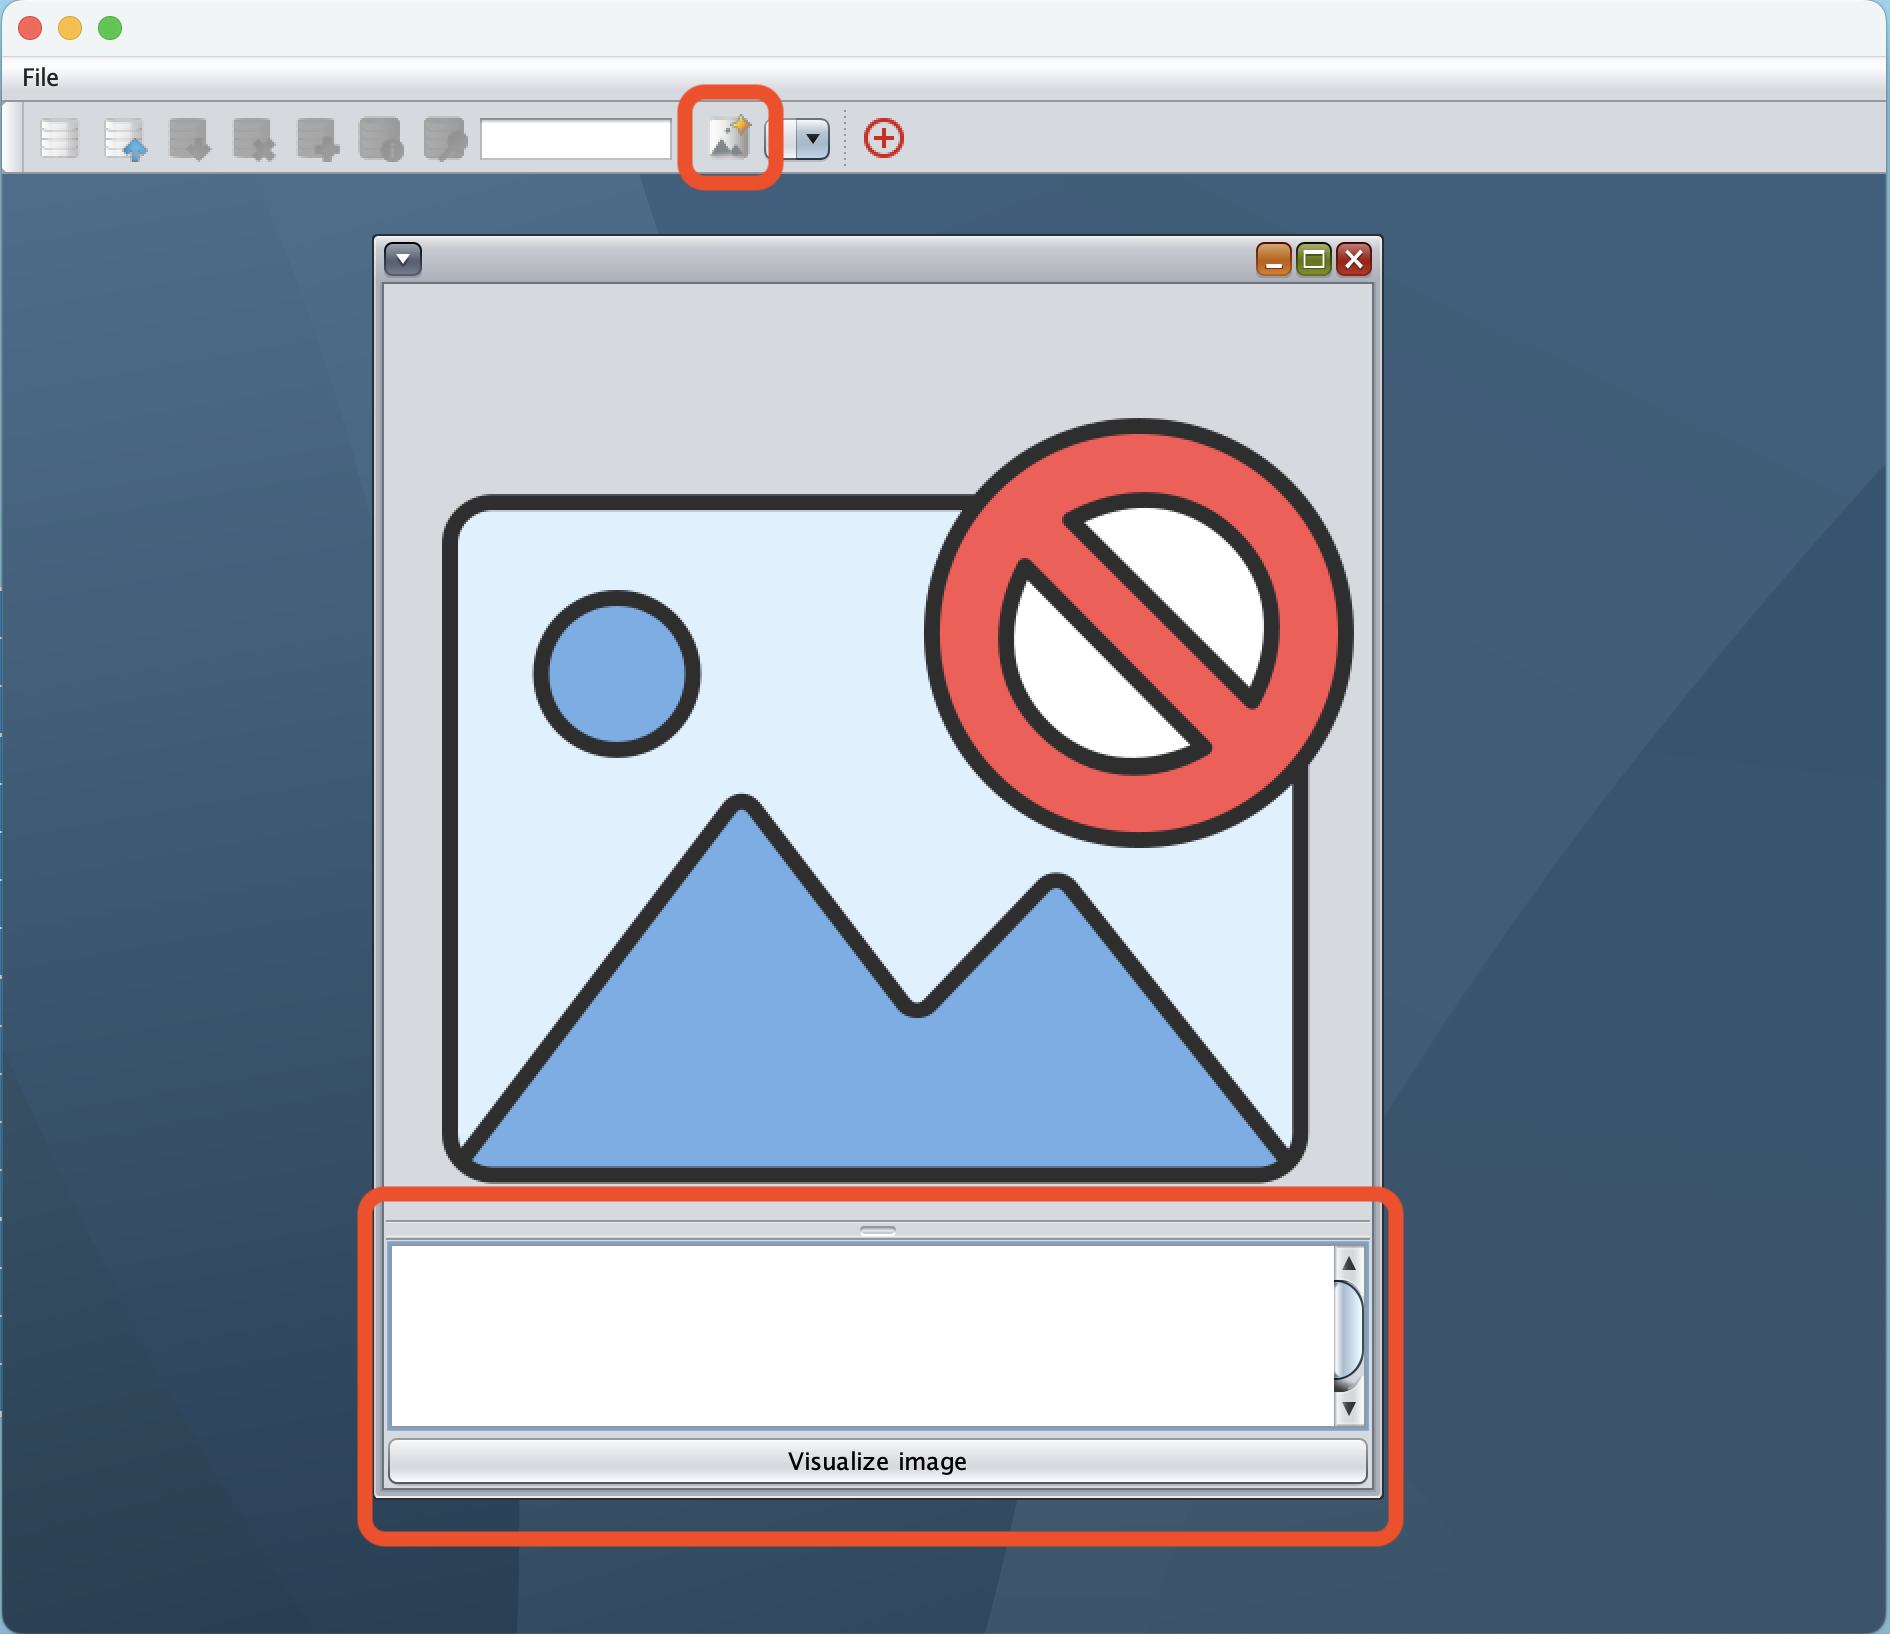
\includegraphics[width=0.5\textwidth]{manual/captura3.png}
        \caption{Ventana interna con área para escribir y botón de visualizar}
        \label{fig:visualizar}
    \end{figure}
\end{enumerate}

\textbf{Paso 2: Escribir la descripción}
\begin{enumerate}
    \item En el cuadro de texto, introduce una descripción lo más detallada posible de la imagen que deseas generar.
    \item Ejemplo: \textit{``A dog running on the beach with its friend.''}
\end{enumerate}

\textbf{Paso 3: Generar y visualizar la imagen}
\begin{enumerate}
    \item Haz clic en el botón \textit{Visualizar Imagen}.
    \item La imagen generada sustituirá a la imagen por defecto en la misma ventana.
    \item Además, la imagen y su descripción se guardarán automáticamente en el historial de generación.
\end{enumerate}

\begin{figure}[H]
    \centering
    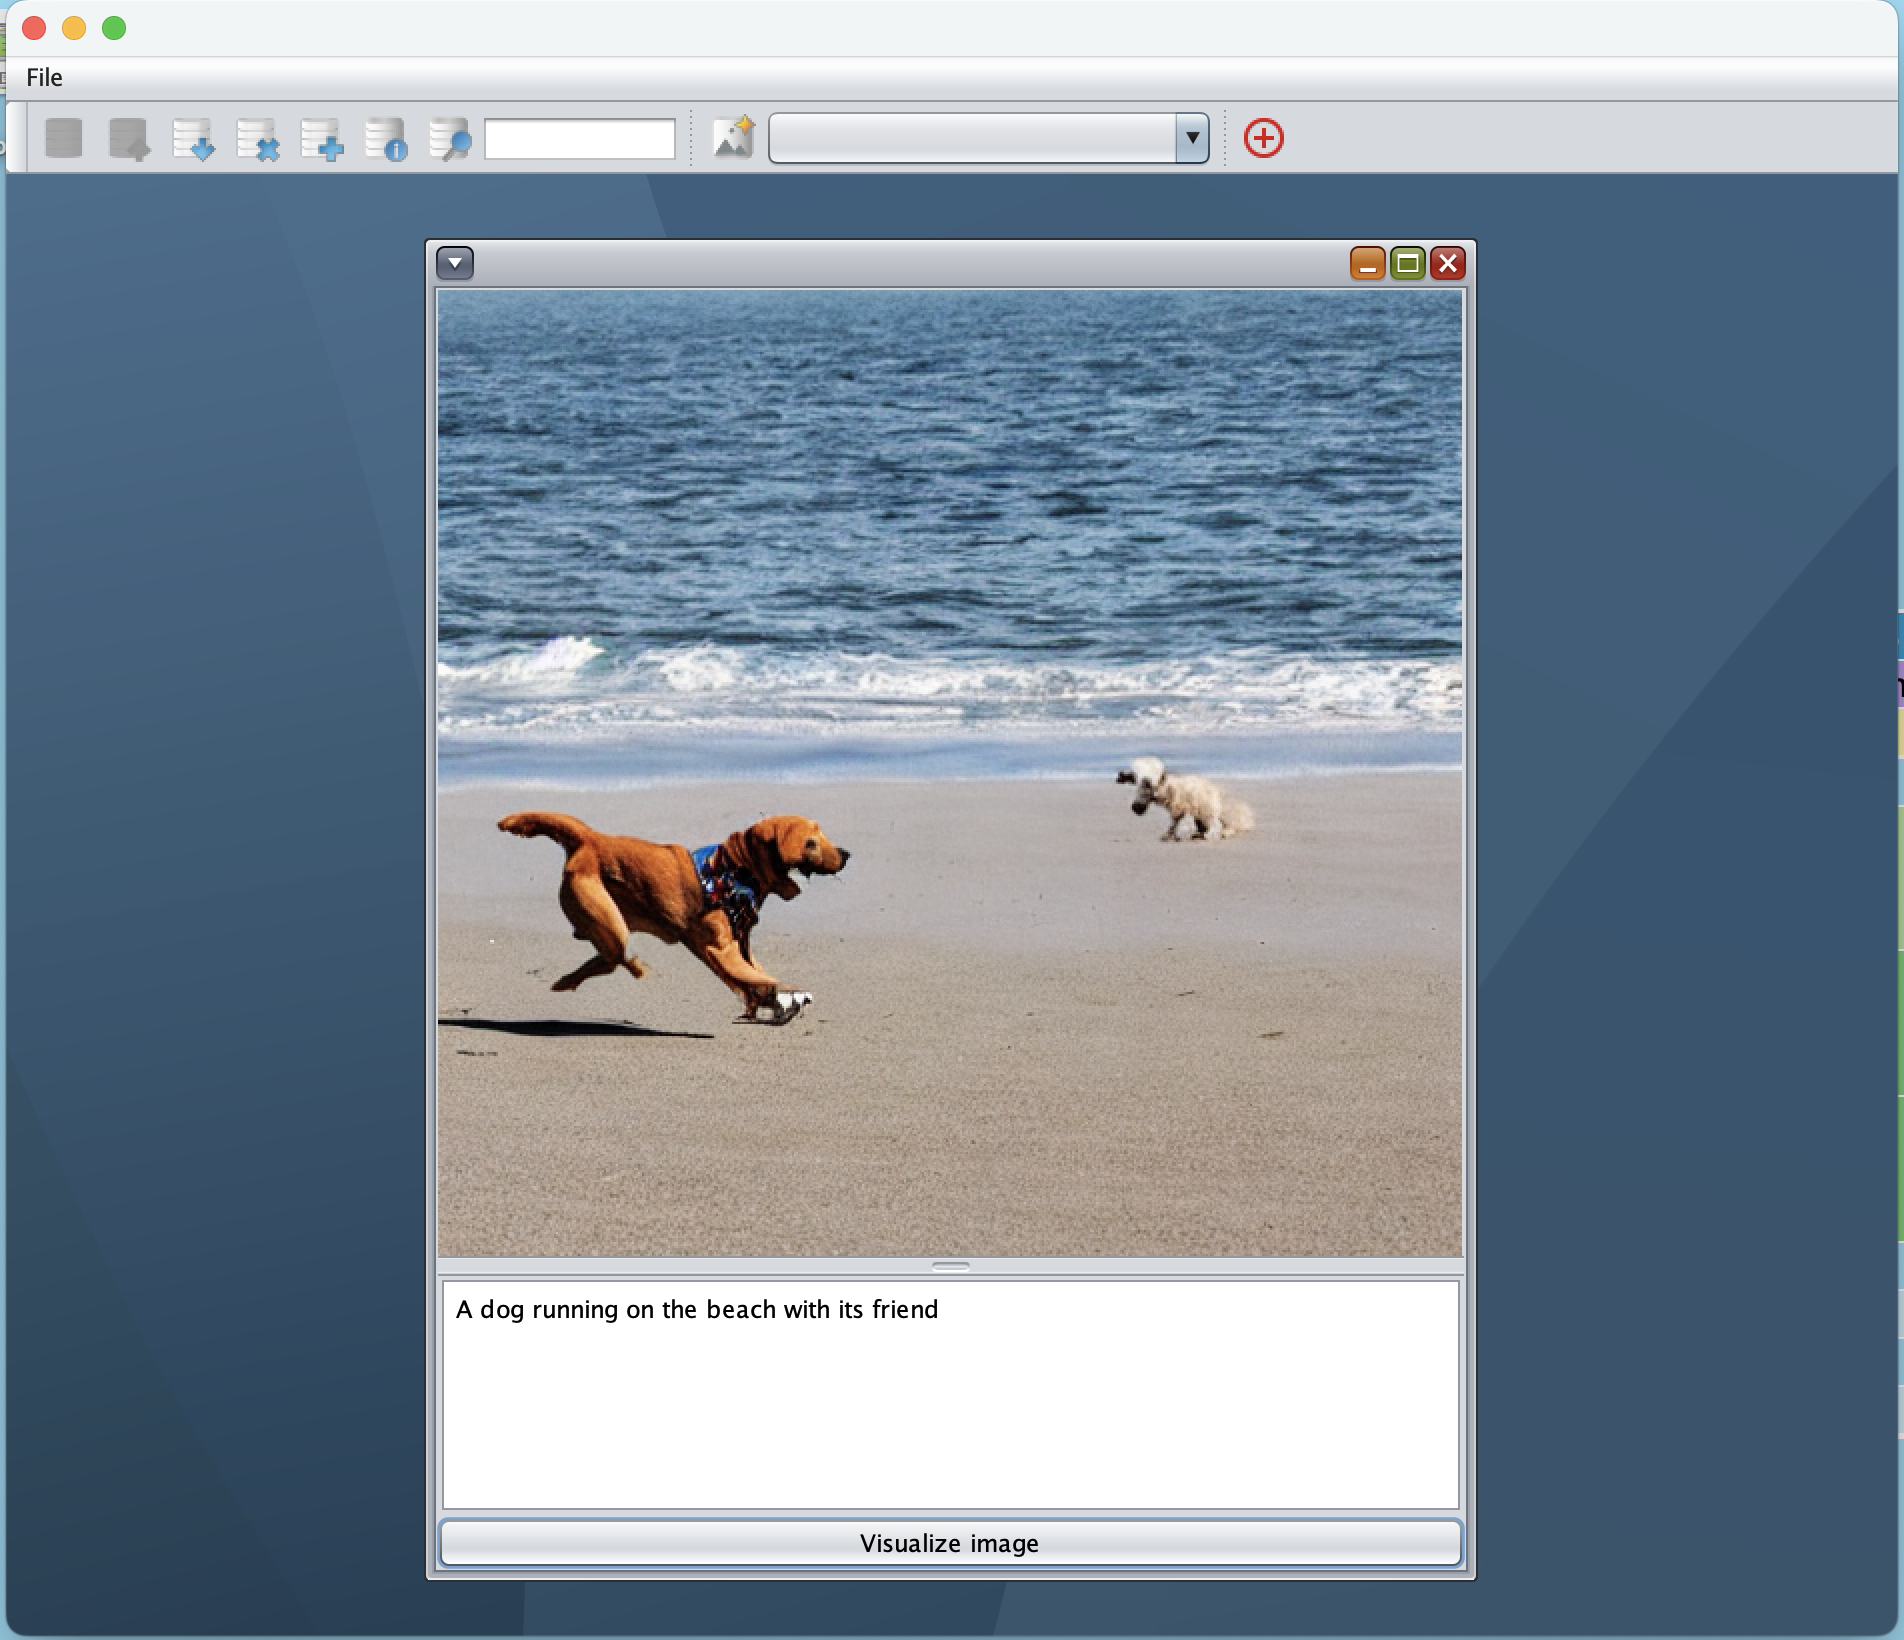
\includegraphics[width=0.5\textwidth]{manual/captura5.png}
    \caption{Ejemplo de visualización}
    \label{fig:ejemplo}
\end{figure}


\subsection{Cómo generar una consulta sin mostrar la imagen}

Esta funcionalidad permite lanzar una consulta basada en una descripción textual sin necesidad de generar ni visualizar la imagen en pantalla. En su lugar, se realiza una búsqueda en la base de datos para recuperar resultados visualmente similares.

\textbf{Paso 1: Escribir la descripción}
\begin{enumerate}
    \item Introduce el texto descriptivo en el cuadro situado en la barra de herramientas superior.
    \item Ejemplo: \textit{"A futuristic city skyline at night with neon lights."}
\end{enumerate}

\begin{figure}[H]
    \centering
    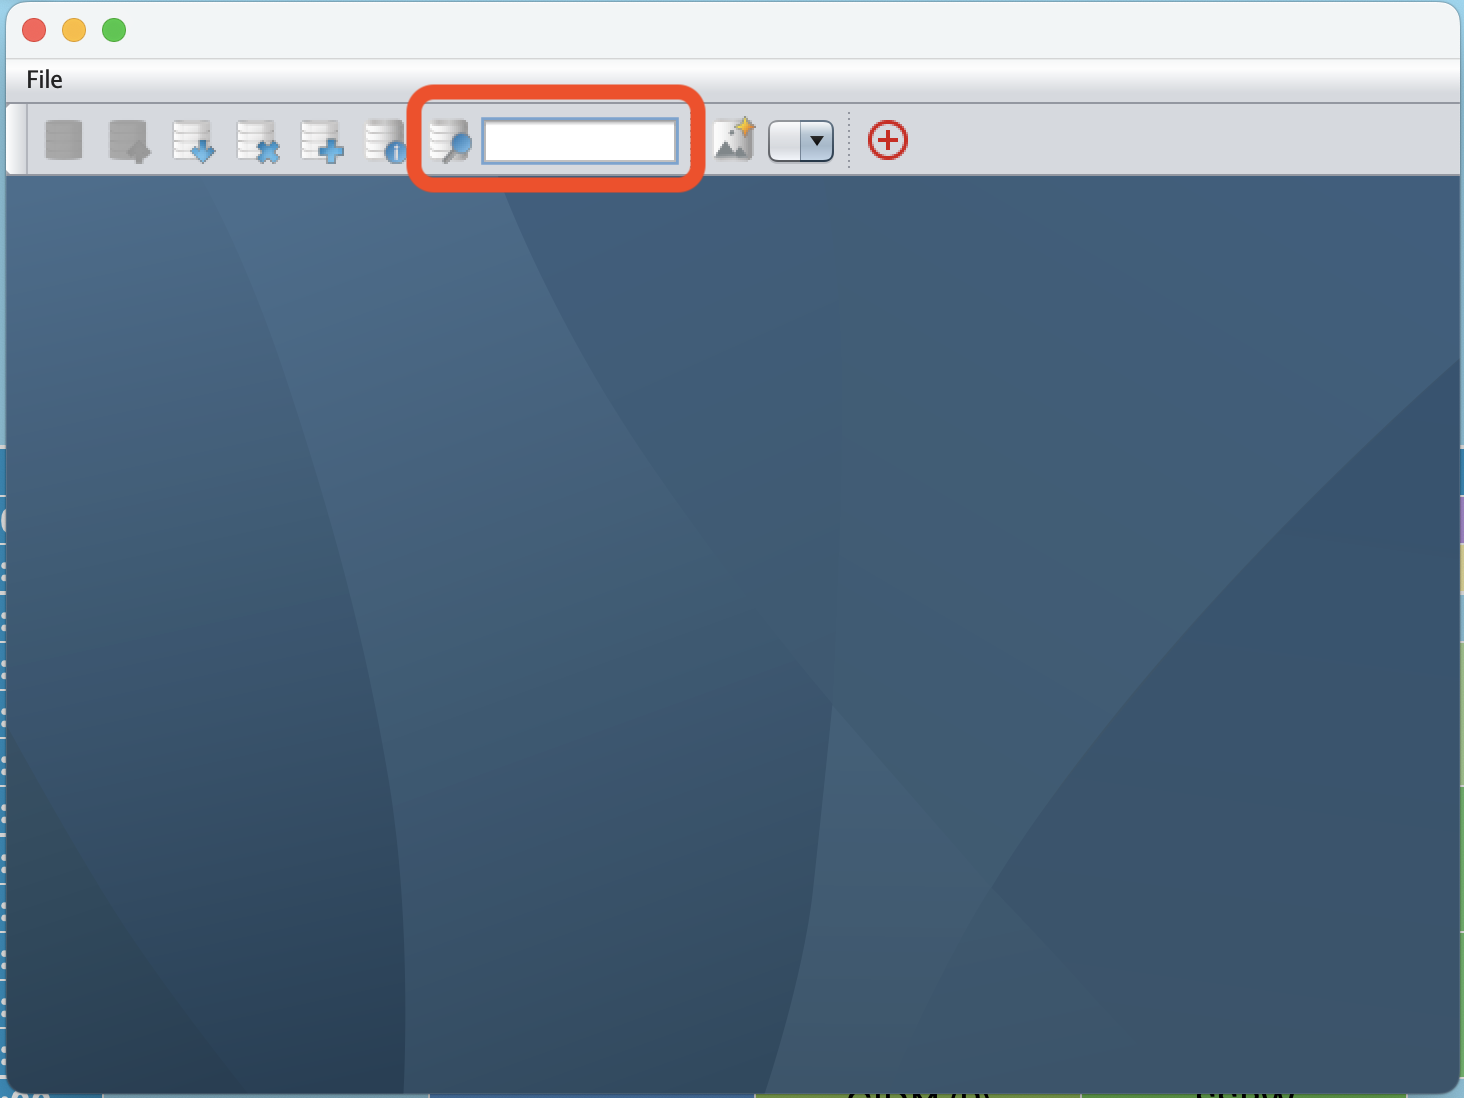
\includegraphics[width=0.5\textwidth]{manual/captura2.png}
    \caption{Escribir la descripción en la barra superior}
    \label{fig:consulta-cuadro}
\end{figure}

\textbf{Paso 2: Ejecutar la consulta}
\begin{enumerate}
    \item Haz clic en el botón de búsqueda situado junto al cuadro de texto.
    \item El sistema generará la imagen en segundo plano y lanzará una búsqueda automática en la base de datos utilizando la imagen como consulta.
\end{enumerate}

\textbf{Paso 3: Visualización de resultados}
\begin{enumerate}
    \item Se abrirá una nueva ventana con los resultados visuales recuperados desde la base de datos, similares a la imagen generada a partir de tu descripción.
\end{enumerate}

\textbf{-- Imagen sugerida: Captura de la ventana de resultados abiertos tras ejecutar la consulta. --}


\subsection{Reutilizar imágenes generadas}
Todas las imágenes generadas se almacenan automáticamente en el historial, junto con la descripción (prompt) que se utilizó para crearlas. Este historial se encuentra accesible mediante una lista desplegable en la parte superior de la interfaz.

Para reutilizar una imagen generada anteriormente:
\begin{enumerate}
    \item Despliega la lista situada en la parte superior.
    \item Selecciona una de las entradas del historial (aparecen truncadas si son largas, pero se muestran completas en su tooltip).
    \item La imagen correspondiente se abrirá en una nueva ventana interna, con el texto de la descripción como título.
\end{enumerate}

\begin{figure}[H]
    \centering
    \begin{minipage}[t]{0.48\textwidth}
        \centering
        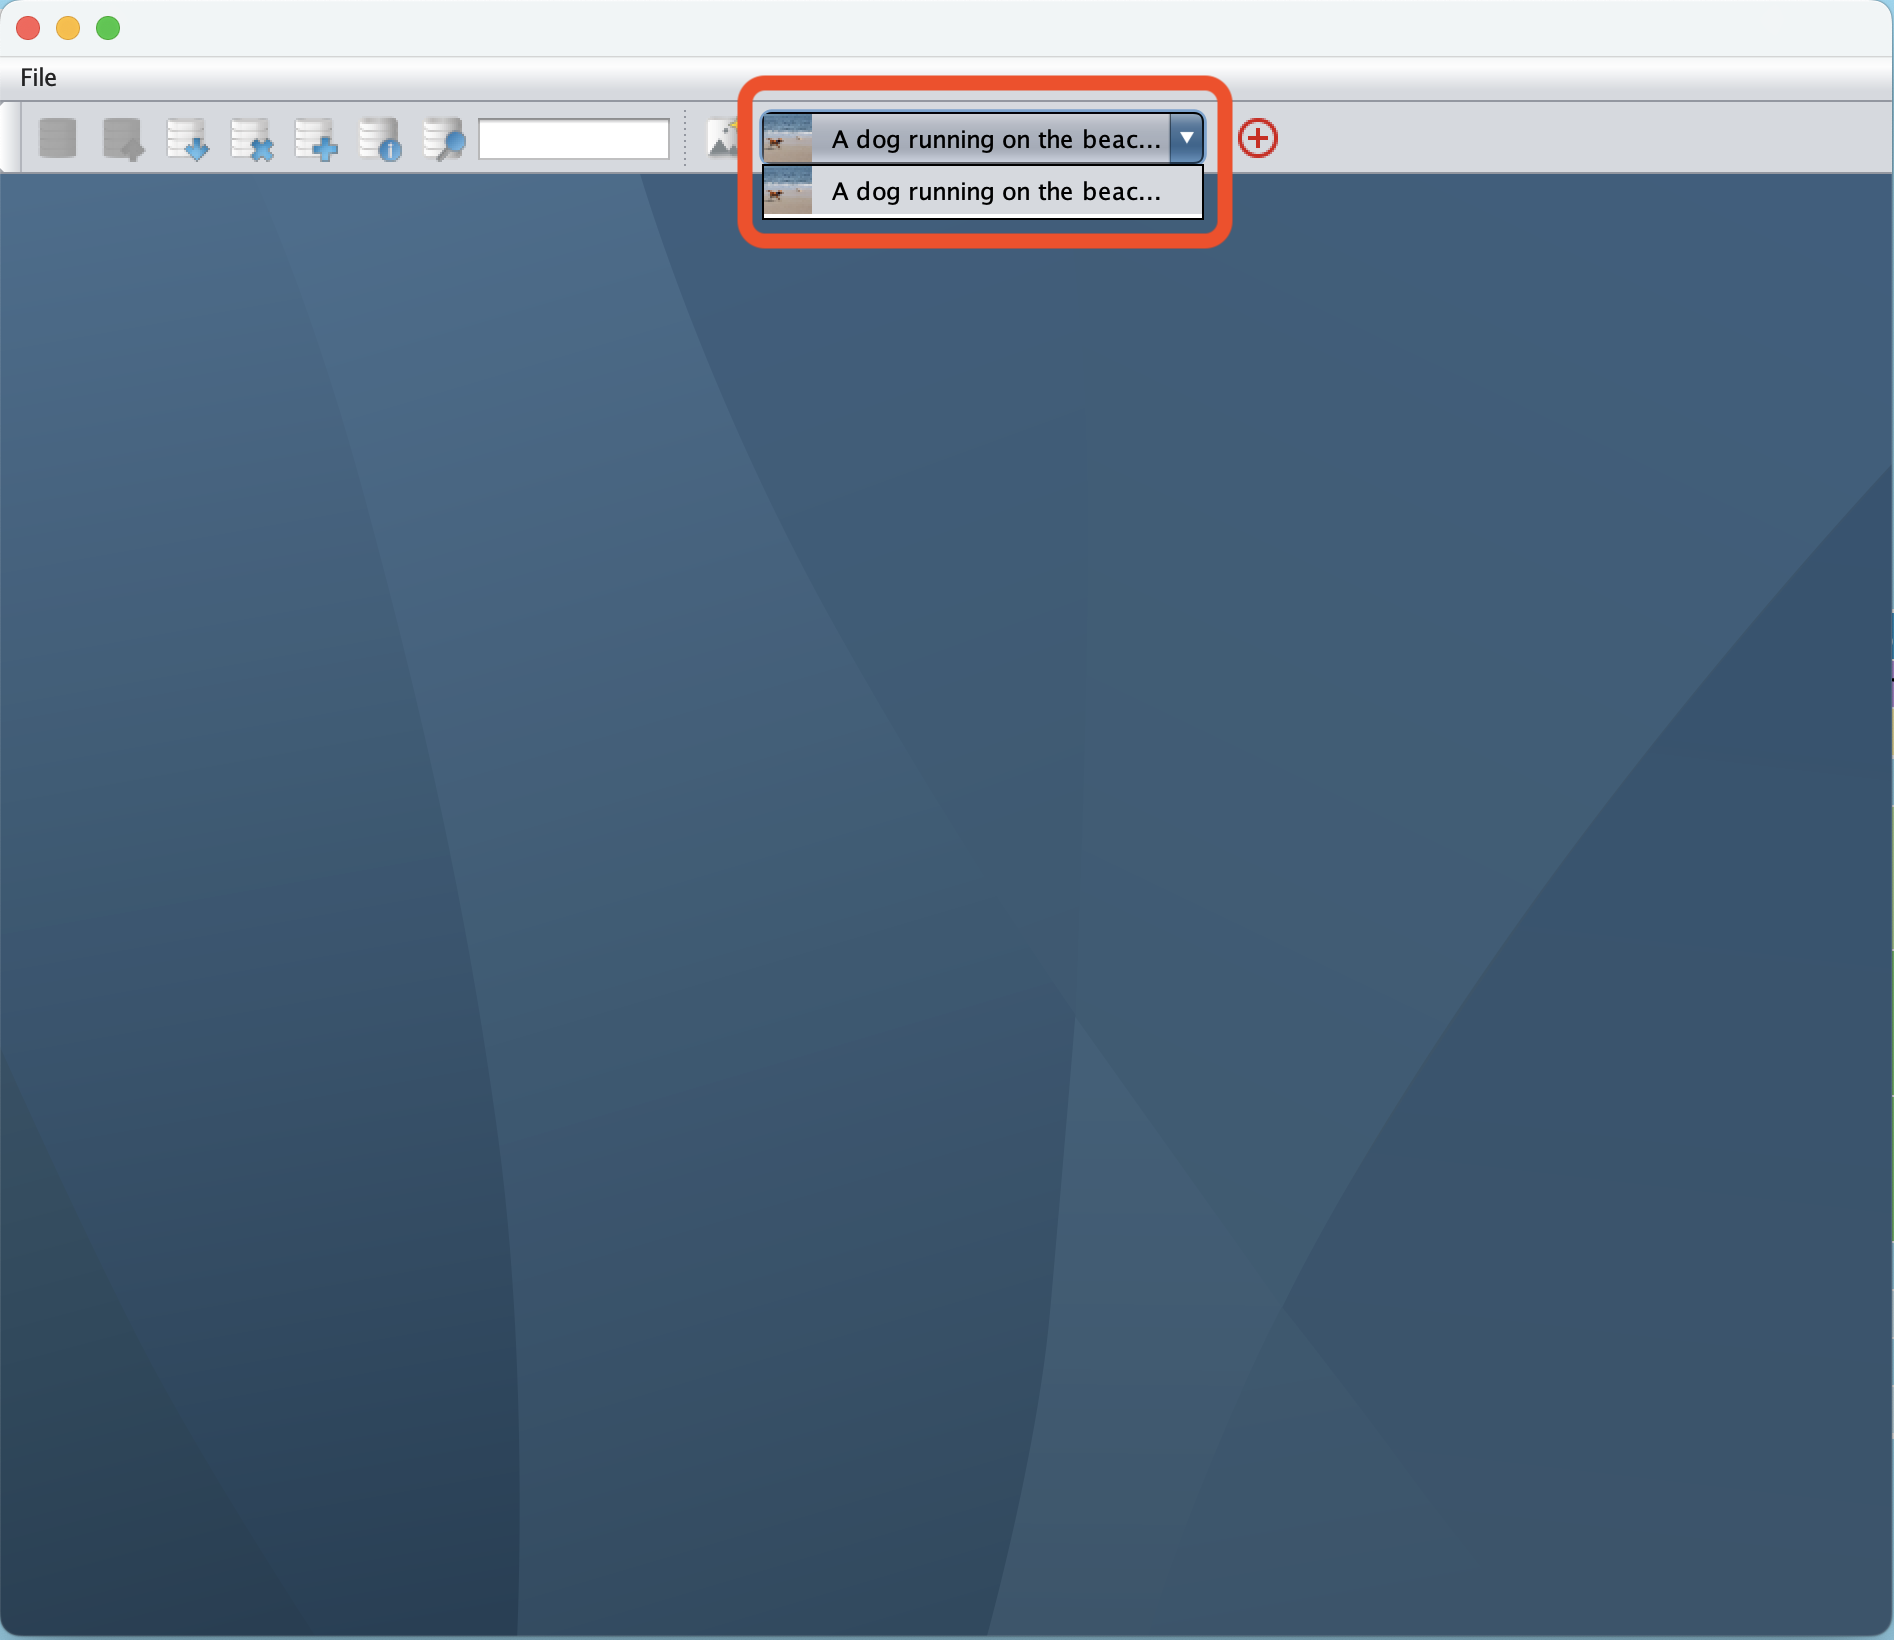
\includegraphics[width=\textwidth]{manual/captura6.png}
    \end{minipage}
    \hfill
    \begin{minipage}[t]{0.48\textwidth}
        \centering
        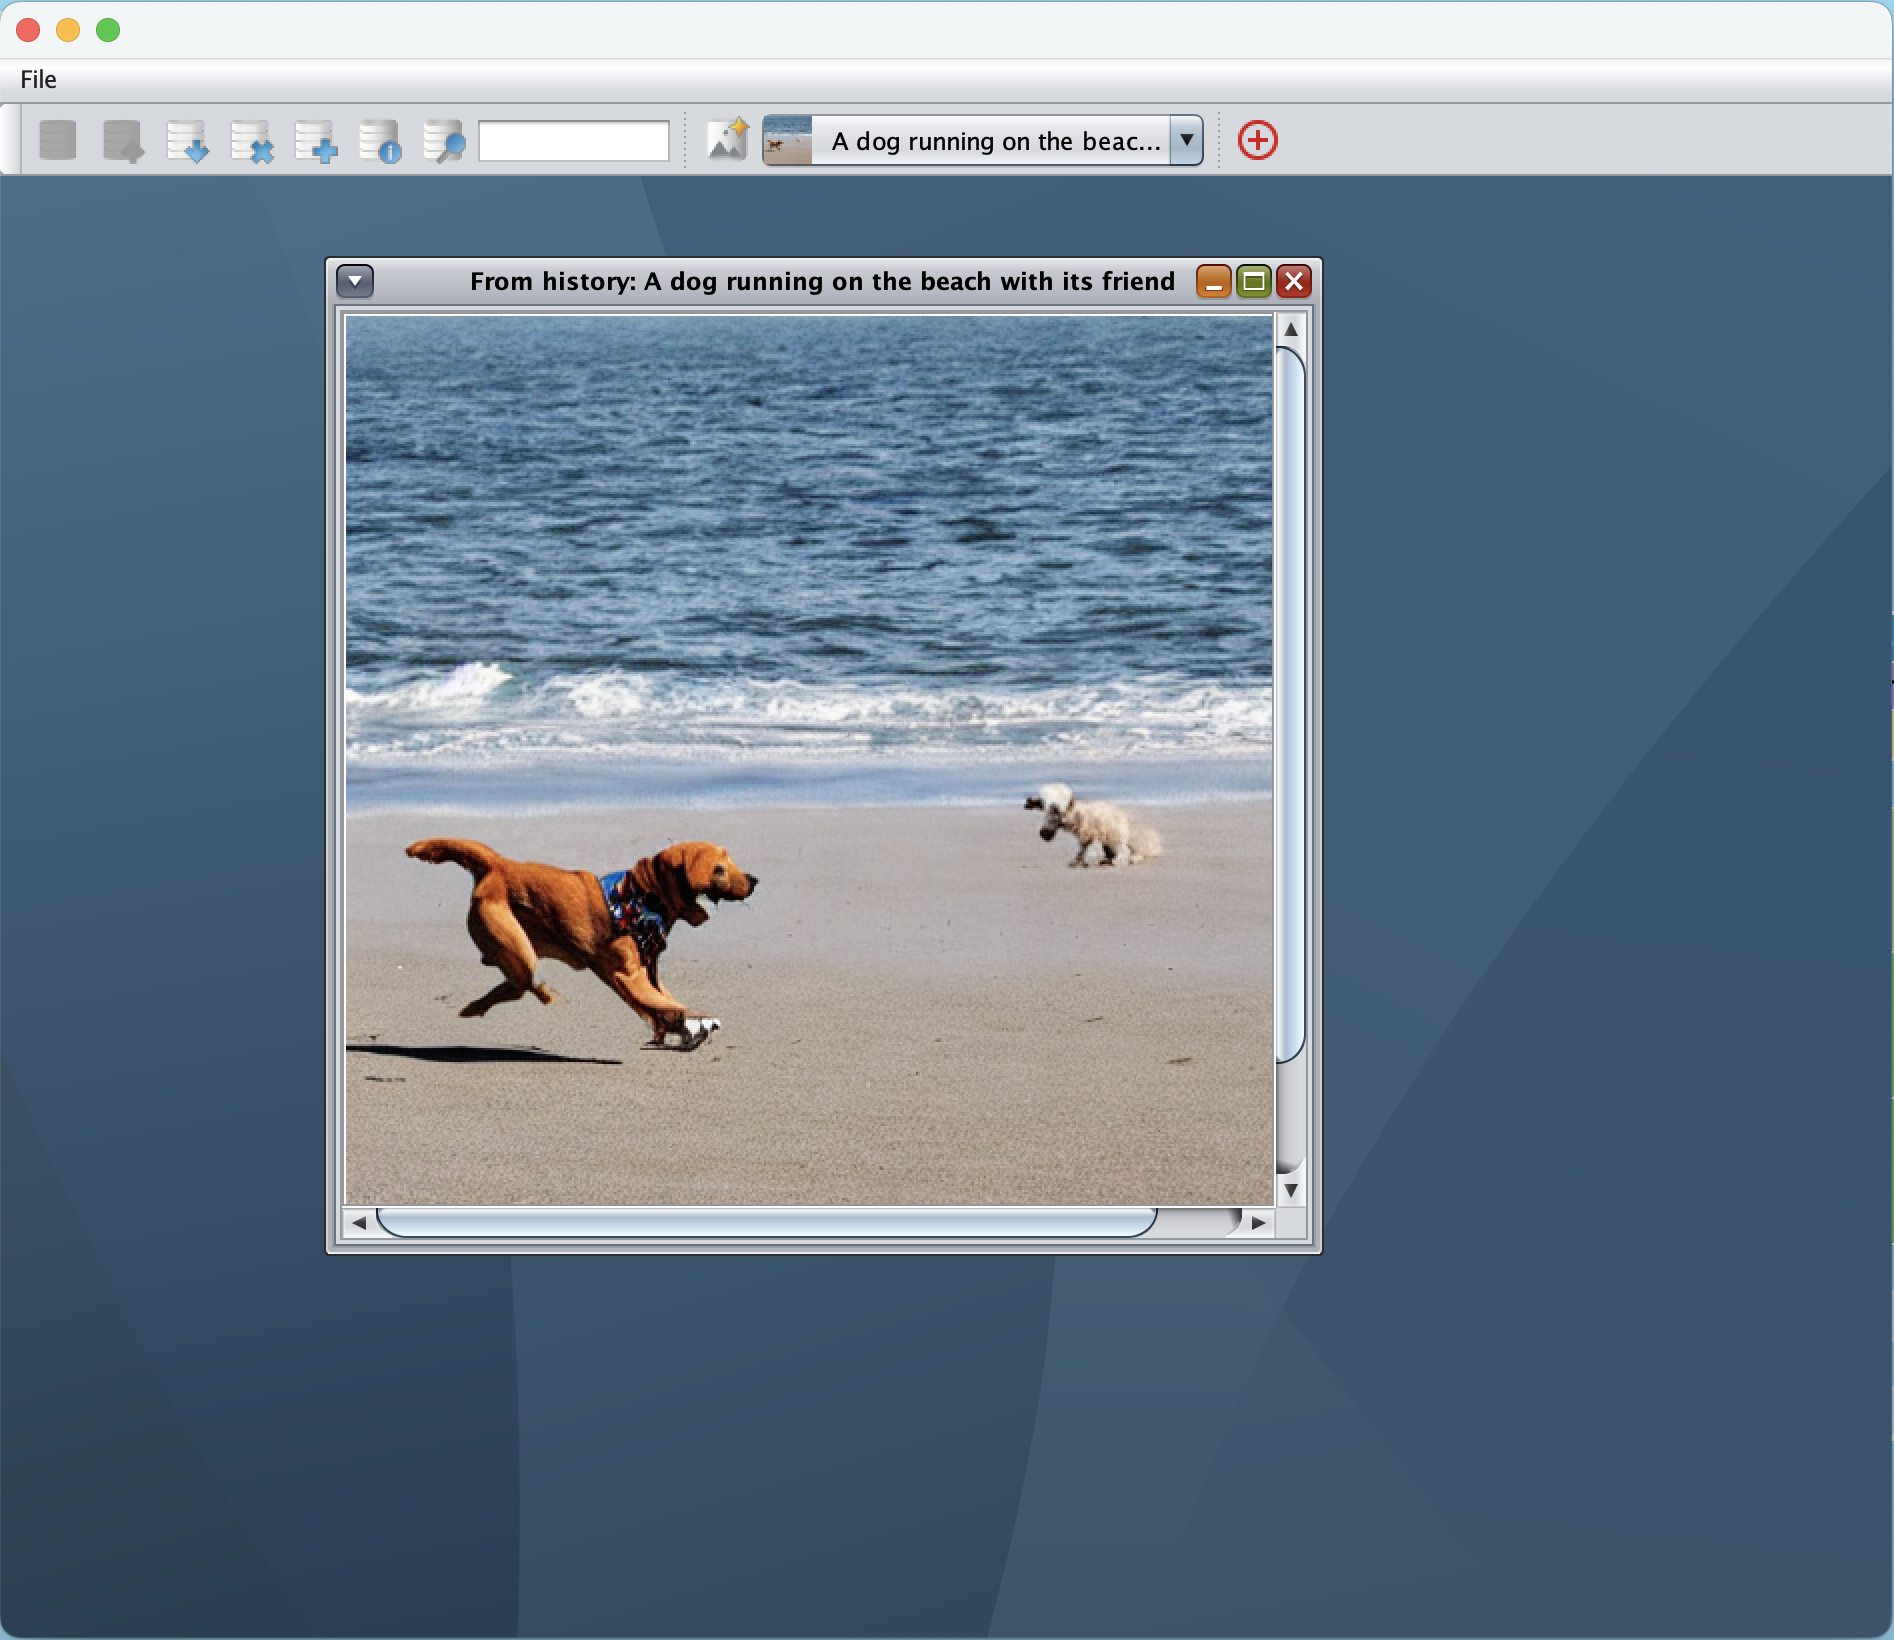
\includegraphics[width=\textwidth]{manual/captura7.png}
    \end{minipage}
    \caption{A la izquierda, vista del historial con una entrada seleccionada. A la derecha, la imagen generada que se abre al seleccionar esa entrada.}
    \label{fig:historial}
\end{figure}


\subsection{Errores y soluciones comunes}

Error al generar la imagen:
Mensaje: "No se pudo generar la imagen. Verifique su descripción."
Solución: Asegúrate de que la descripción ingresada sea clara y contenga suficiente detalle.
Error al cargar el modelo:
Mensaje: "El modelo seleccionado no es compatible."
Solución: Verifica que el archivo sea un modelo compatible con la aplicación.
Imagen sugerida: Capturas de ejemplos de mensajes de error y su ubicación en la interfaz.